\documentclass{CourseOutline}

\SetDate[09/01/2023]

\logo{img/CONU-logo-clr.png}

\Course{COEN 244}{S}{Programming Methodology II}{M/W}{13:15-14:30}{MB 1.210}
\Semester{Fall 2021}{Jan 9th}{Apr 17th}
\Prof{Stuart Thiel}{stuart.thiel@gmail.com}{Zoom, by appointment}[img/stuart.jpg]



\begin{document}

\maketitle
  

\vspace{10mm}

%
% Remember to check this for the current semester!
%
% https://byblos.encs.concordia.ca/CoursePages/Courses.vm?acyear=2018&term=1

\begin{courseblock}
\tutorial{Th, 16:15-17:55}{H 907}{Mina Masoumi}[minamasoomi31@gmail.com]
\tutorial{Th, 16:15-17:35}{H 847}{Ismael Ridha}[ismaelmergasori@gmail.com]
\tutorial{F, 16:15-17:55}{H 917}{Mustafa Daraghmeh}[mustafa.daraghmeh@concordia.ca]
\tutorial{F, 16:15-17:55}{H 843}{Zaedul Islam}[islam.zaedul@gmail.com]\addtocounter{TutorialSection}{2}%
\tutorial{Th, 16:05-17:45}{H 903}{Zaedul Islam}[islam.zaedul@gmail.com]
\marker[Mohammad Reza Rejali][mohammadreza.rejali@concordia.ca]
\marker[Ismael Ridha][ismaelmergasori@gmail.com]
\end{courseblock}

% Course details
\section{Description}
\textbf {\large \\ Course Description:} Review of object-oriented programming and further concepts. More on classes. Revisiting pointers. Operator overloading: regular and advanced usage. Fundamentals of file and stream processing. Class composition and inheritance: regular and advanced usage. Virtual functions. Polymorphism. Static and dynamic binding. Abstract classes. Case study of a small-scale object-oriented project: simplified analysis, design, and implementation. Introduction to templates, the standard template library, and exception handling. Introduction to dynamic data types. Namespaces. Lectures: three hours per week. Tutorial: two hours per week.
NOTE: Students who have received credit for COMP 249 may not take this course for credit.

\section{Course Details}

\textbf {Prerequisite:} COEN 243 \\

\textbf {This course is a prerequisite to::} \\

\textbf {\large Text(s):} C++ How to Program (10th Edition) \\
\textbf {Author(s):} Paul Deitel and Harvey Deitel; \\ 
\textbf {ISBN-10:} 0-13-444823-5 \\ 
\textbf {ISBN-13:} 978-0-13-444823-7 \\ 
\textbf {Online Resources:} \url{http://www.deitel.com/Books/C/CHowtoProgram10e/tabid/3678/Default.aspx} \\


\textbf {Knowledge base for engineering prerequisites}\\
This course requires knowledge in:
\begin{enumerate}
    \item Programming logic, C++
    \item Object-oriented programming basics, C++
\end{enumerate}


% I recommend using \newpage here if necessary
\textbf {\large Grading Scheme:} \\
\hspace*{40mm}
\begin{tabular}{ l l }
Individual Assignments x 3 & 20\% \\
Midterm & 30\% \\
Final & 50\% \\
\end{tabular} \\\\

\textbf {Assignments:} 
Assignments will be individual. Your best two assignments will be worth 7\% each; the other one will be worth 6\%. Late submissions will not be graded. Assignment submission will be through EAS (\url{https://fis.encs.concordia.ca/eas/}). \\

\textbf {Midterm:} There will be a midterm. It will be in-class and it will be Multiple-Choice/Multiple-Answer format.\\

\textbf {Final:} There will be a final, with timing set by the University.  It will be in-person and it will be Multiple-Choice/Multiple-Answer format.\\

\textbf {\large Letter Grade Distribution:} Grades will be curved around a B,
unless the class does abysmally as a whole, then it will be curved around a B-.
1.8 standard deviations below the mean is the threshold to FAIL. Two standard
deviations above is a guaranteed A+. \\

\textbf {\large \\ Plagiarism:}\\
The most common offense under the Academic Code of Conduct is plagiarism, which the Code defines as "the presentation of the work of another person, in whatever form, as one's own or without proper acknowledgement" (Article 19a). \footnote{ \url{www.concordia.ca\students\academic-integrity\plagiarism.html}, May 4th, 2017 }

It's not hard, don't cheat. Don't copy other people's code. Don't copy code off the Internet and pass it off as your own (or for this course, just don't copy code off the Internet).

\newpage

% Course Outline
\begin{DetailedOutline}{Course Outline - First Half}
\LectureEntry[0]{
    Course Description \textbf{\small Outline}
}
\LectureEntry[2]{
    \textbf{Live-Coding} \\
    Overview of C++ (main function, cin/cout, variables and constants, arrays, enumerated types, If-else, loops, strings, functions, pointers, namespaces, structures) \textbf{Ch. 1‐8 (COEN 243 Concepts)} \\
    Making tic-tac-toe}
\LectureEntry[5]{
    C++ Classes (Data abstraction, classes and objects, encapsulation, data members, function members, constructors and destructors) \textbf{Ch. 3, 9}
}
\LectureEntry[2]{
    \textbf{Live-Coding} \\
    Examples, an object-oriented approach \\
    Making tic-tac-toe Object-Oriented
}
\LectureEntry[5]{
    C++ Classes (Pointers revisited, dynamic memory allocation, object references, static members, copy constructors) \textbf{Ch. 3, 9}
}
\LectureEntry[2]{
    \textbf{Live-Coding} \\
    Examples with dynamic memory allocation in classes \\
    Making tic-tac-toe support dynamic board sizes
}
\LectureEntry[5]{
    Class Composition \textbf{Ch. 9}
}
\LectureEntry[2]{
    \textbf{Live-Coding} \\
    Class Composition (case study) – Modeling Class Composition in UML \\
    \textbf{Course Material} \\
    Drawing Shapes Example : Composite Shapes
}
\LectureEntry[5]{
    Class Inheritance (Software reuse, class reuse, the is-a rule, "protected" members, base and derived classes, types of inheritance, constructors, and destructors under inheritance) \textbf{Ch. 11}
}
\LectureEntry[2]{
    Polymorphism (static and dynamic binding, function overloading, function overriding, virtual functions, virtual destructors) \textbf{Ch. 12}
}
\LectureEntry[5]{
    \textbf{Live-Coding} \\
    Examples with inheritance \\
    Drawing Shapes Example: Applying Inheritance
}
\LectureEntry[2]{
    More Polymorphism (pure virtual functions, pure abstract classes) \textbf{Ch. 12}
} 
\LectureEntry[5]{
    \textbf{Live-Coding} \\
    Examples with polymorphism \\
    Drawing Shapes Example : Applying Polymorphism
}
\LectureEntry[2]{
    Midterm - All material till here
} 
\LectureEntry[5]{
    Midterm Break
}[gray!25]
\LectureEntry[2]{
    Midterm Break
}[gray!25]
\end{DetailedOutline}

\newpage

\begin{DetailedOutline}{Course Outline - Second Half}
\LectureEntry[5]{
    Operator Overloading (Introduction, overloading arithmetic operators) \\
    \textbf{Ch. 10}
}
\LectureEntry[2]{
    \textbf{Live-Coding} \\
    Examples of operator overloading, static and as member operations, implicit casting \\
    Shapes Example: Composite Shapes by adding shapes
}
\LectureEntry[5]{
    Advanced Exception Handling (user-defined exceptions, exception \\
    propagation) \textbf{Ch. 17}
}
\LectureEntry[2]{
    \textbf{Live-Coding} \\
    Examples of exception handling \\
    Revisiting tic-tac-toe to add exceptions
} 
\LectureEntry[5]{
    Advanced Input/Output in C++ \textbf{Ch. 13, 14}
}
\LectureEntry[2]{
    Templates (Class templates, template instantiation, type \\
    binding) \textbf{Ch. 18}
}
\LectureEntry[5]{
    \textbf{Live-Coding} \\
    Examples with IO Manipulators, \texttt{array} and \texttt{vector} containers and iterators
}
\LectureEntry[2]{
    Introduction to Data Structures, Standard Template Library, and Algorithms \textbf{Ch. 15, 16}
}
\LectureEntry[5]{
    Problem Analysis \textbf{Course Material} \\
    Lambdas
}
\LectureEntry[2]{
    \textbf{Live-Coding} \\
    Examples of algorithms library and lambdas
}
\LectureEntry[5]{
    Easter Holiday
}[gray!25]
\LectureEntry[2]{
    \textbf{Live-Coding} \\
    Examples: combing array/vector with the algorithms library and lambdas
}
\LectureEntry[5]{
    Review \textbf{\small Ch. Notes}\\
}
\LectureEntry{
    Final - Both halves of the course
}[gray!25]
\end{DetailedOutline}

The general flow of the course outline may change, but only slightly at this point. \\

\newpage
\includegraphics[page=3,rviewport=0.11 0.05 0.9 0.96, scale=0.95, clip=true]{2022_COEN244_4_S_1_outline.pdf}
\newpage
\includegraphics[page=4,rviewport=0.11 0.05 0.9 0.96, scale=0.95, clip=true]{2022_COEN244_4_S_1_outline.pdf}
\newpage
\includegraphics[page=5,rviewport=0.11 0.05 0.9 0.96, scale=0.95, clip=true]{2022_COEN244_4_S_1_outline.pdf}

\end{document}
